\documentclass[12pt]{article}

% report, book

%  Русский язык

\usepackage[T2A]{fontenc}
\usepackage[utf8]{inputenc}
\usepackage[english,russian]{babel}

\usepackage{amsmath,amsfonts,amssymb,amsthm,mathtools} 

\usepackage{graphicx}
\usepackage{listings}
\usepackage{hyperref}
\usepackage[table,xcdraw]{xcolor}

\usepackage{wasysym}

\usepackage{geometry} 
\geometry{a4paper,top=2cm,bottom=3cm,left=2cm}

\begin{document}

\begin{titlepage}
   \begin{center}
       \vspace*{1cm}

       \textbf{Лабораторная работа №2}

       \vspace{0.5cm}
        Алгоритмы многомерной минимизации функции
            
       \vspace{1.5cm}

       \textbf{Сысоев Александр, Зырянова Мария}
       
       \textbf{Верблюжий случай}

       \vfill
            
   \end{center}
\end{titlepage}

% TODO:
% генерирование n-мерных приколов
% линии уровня


\section{Постановка задания}

Требуется реализовать алгоритмы поиска минимума функции нескольких переменных, исследовать их, оценить поведение:
\begin{itemize}
\item метод градиентного спуска
\item метод наискорейшего спуска
\item метод сопряженных градиентов
\end{itemize}

Ограничение на исследуемые функции -- они должны быть квадратичными, то есть представимы в виде
\[ f(x) = f(x_1, x_2, \cdots, x_n) = \frac{1}{2} \sum_{i, j = 1}^n a_{ij} x_i x_j - \sum_{i=1}^n b_i x_i + c\].

В матричной форме эти функции имеют вид:
\[ f(x) = \frac{1}{2} x^T Ax - b^Tx + c  \text{, где } x = (x_1, \cdots, x_n)^T, b = (b_1, \cdots, b_n)^T \]

\section{Предварительное исследование}

Основная задача -- найти минимум заданной функции. По теореме Ферма, если точка $x^*$ -- минимум функции, то $f'(x^*) = 0$. В многомерном случае можно применить этот критерий последовательно к каждой частной производной, и тогда получится критерий минимума функции нескольких переменных -- равенство всех частных производных нулю. Величина, за это отвечающая -- градиент, то есть если $x^* = (x_1^*, \cdots, x_n^*)$ -- минимум функции, то
\[ \nabla f(x^*) = 0 \]

Рассмотрим частную производную по $x_i$ квадратичной функции:
\[ \frac{\delta}{\delta x_i}f(x_1, \cdots, x_n) = a_{ii}x_i + \sum_{j \neq i} \frac{1}{2} (a_{ij}+a_{ji})x_j - b_i \]

То есть в общем виде градиент квадратичной функции выглядит следующим образом:
\[ \nabla f(x) = Ax-b \]

$A$ -- симметричная матрица ($\Rightarrow$ ее можно рассматривать, как треугольную), у которой на пересечении $i$ строки и $j$ столбца стоит величина $\frac{1}{2}(a_{ij}+a{ji})$.

В случае, если градиент в точке не равен нулю, он показывает направление наибольшего локального увеличения функции. Поэтому, если двигаться в направлении антиградиента (то есть $-\nabla f(x)$), то будет происходить движение в направлении убывания $f(x)$.

\section{Исследуемые функции}

Для анализа методов были выбраны следующие квадратичные функции:
\begin{enumerate}

\item \[ f(x) = 64x_1^2 + 126x_1x_2 + 64x_2^2 - 10x_1 + 30x_2 + 13 \]
\begin{figure}[h]
	\centering
	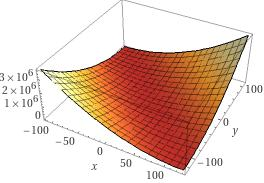
\includegraphics[scale=0.5]{img/func1_plot.jpeg}
	\caption{График функции.}
\end{figure}

\begin{figure}[h]
	\centering
	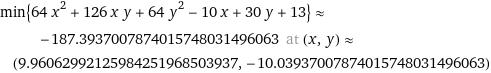
\includegraphics[width=0.5\textwidth]{img/func1_min.jpeg}
	\caption{Минимум, найденный с помощью Wolphram Alpha.}
\end{figure}

\end{enumerate}

\newpage
\section{Метод градиентного спуска}

Как было написано ранее, двигаясь в направлении антиградиента, функция убывает. То есть по точке $x^k$ можно получить точку $x^{k+1}$ с меньшим значением функции $f$. Повторяя это нескольно раз, построится последовательность $x^{k+1} = x^{k} - \alpha^{k} \nabla f(x^k)$. При этом, $\alpha_k$ (величина шага) такова, что $f(x^{k+1}) < f(x^k)$.  

Точка является миниумом, если в ней квадратичная форма положительно определена. Матрица $A$ -- симметричная, будем считать, что положительно определенная. Пусть $L$ -- наибольшее собственное значение $A$, тогда при любых $\alpha \in \left(0; \frac{2}{L} \right)$ и $x$ из области определения фукнции $x^{k+1} = x^{k} - \alpha^{k} \nabla f(x^k)$, будет сходиться к единственной точке глобального минимума $x^*$ линейно, со скоростью геометрической прогрессии. В этом случае последовательность $x_k$ будет релаксационной и не будет происходить "проскакивания" стационарной точки.

Таким образом, посчитав максимальное собственное число $A$, примем $\alpha = \frac{2}{L}$, и затем будем выстраивать последовательность. Если на каком-то шаге $f(x^{k+1}) \geqslant f(x^k)$, то был сделан слишком большой шаг и следует уменьшить $\alpha$. Примем новое $\alpha = \frac{\alpha}{2}$. Будем повторять до условия остановки: $\lVert \nabla f(x^k) \rVert \leqslant \epsilon$, либо до указанного колчиества итераций, если это было дано (в нашем исследовании -- 2000).

% Please add the following required packages to your document preamble:
% \usepackage[table,xcdraw]{xcolor}
% If you use beamer only pass "xcolor=table" option, i.e. \documentclass[xcolor=table]{beamer}
\begin{table}[h]
\begin{tabular}{|c|c|c|c|c|c|c|}
\hline
\rowcolor[HTML]{FFF0DB} 
\cellcolor[HTML]{FFF0DB}\textbf{$\epsilon$} &
  \textbf{$x_1$} &
  \textbf{$x_2$} &
  \textbf{\begin{tabular}[c]{@{}c@{}}Количество\\ итераций\end{tabular}} &
  \textbf{\begin{tabular}[c]{@{}c@{}}Значение\\ минимума\end{tabular}} &
  \textbf{$x_{1_{min}}$} &
  \textbf{$x_{2_{min}}$} \\ \hline
$10^{-2}$ & 10 & 10 & 876  & -187.39370078722567 & 9.9606205571591   & -10.039360714639415 \\ \hline
$10^{-2}$ & 10 & 11 & 874  & -187.393700787196   & 9.960619771803191 & -10.039359929283508 \\ \hline
$10^{-2}$ & 11 & 10 & 875  & -187.39370078723766 & 9.9606208830298   & -10.039361040510116 \\ \hline
$10^{-2}$ & 11 & 11 & 854  & -187.39370078704826 & 9.960616643413074 & -10.03935680089339  \\ \hline
$10^{-3}$ & 10 & 10 & 876  & -187.39370078722567 & 9.9606205571591   & -10.039360714639415 \\ \hline
$10^{-3}$ & 10 & 11 & 874  & -187.393700787196   & 9.960619771803191 & -10.039359929283508 \\ \hline
$10^{-3}$ & 11 & 10 & 875  & -187.39370078723766 & 9.9606208830298   & -10.039361040510116 \\ \hline
$10^{-3}$ & 11 & 11 & 854  & -187.39370078704826 & 9.960616643413074 & -10.03935680089339  \\ \hline
$10^{-4}$ & 10 & 10 & 876  & -187.39370078722567 & 9.9606205571591   & -10.039360714639415 \\ \hline
$10^{-4}$ & 10 & 11 & 874  & -187.393700787196   & 9.960619771803191 & -10.039359929283508 \\ \hline
$10^{-4}$ & 11 & 10 & 875  & -187.39370078723766 & 9.9606208830298   & -10.039361040510116 \\ \hline
$10^{-4}$ & 11 & 11 & 854  & -187.39370078704826 & 9.960616643413074 & -10.03935680089339  \\ \hline
$10^{-5}$ & 10 & 10 & 2000 & -187.3937007873267  & 9.960623763053757 & -10.039363920534072 \\ \hline
$10^{-5}$ & 10 & 11 & 2000 & -187.39370078732998 & 9.960623897700582 & -10.039364055180897 \\ \hline
$10^{-5}$ & 11 & 10 & 2000 & -187.39370078732367 & 9.960623641492967 & -10.039363798973282 \\ \hline
$10^{-5}$ & 11 & 11 & 2000 & -187.393700787349   & 9.960624748480237 & -10.039364905960552 \\ \hline
$10^{-6}$ & 10 & 10 & 2000 & -187.3937007873267  & 9.960623763053757 & -10.039363920534072 \\ \hline
$10^{-6}$ & 10 & 11 & 2000 & -187.39370078732998 & 9.960623897700582 & -10.039364055180897 \\ \hline
$10^{-6}$ & 11 & 10 & 2000 & -187.39370078732367 & 9.960623641492967 & -10.039363798973282 \\ \hline
$10^{-6}$ & 11 & 11 & 2000 & -187.393700787349   & 9.960624748480237 & -10.039364905960552 \\ \hline
\end{tabular}
\end{table}

%Число итераций зависит от минимального и максимального собственного значения матрицы.

\newpage
\section{Метод наискорейшего спуска}

Это модификация предудщего метода, в которой коэффициент $\alpha$ каждый раз пересчитывается. После вычисления в начальной точке градиента, движение в направлении антиградиента делается не маленькими шагами, а до тех пор, пока функция убывает. При достижении минимума на выбранном направлении, снова вычисляется градиент функции и описанные действия повторяются.

На каждом $k$-ом шаге коэффициент $\alpha_k$ находится из решения задачи одномерной оптимизации:
\[ \Phi_k (\alpha_k) \rightarrow min, \quad  \Phi_k (\alpha_k) = f(x^k - \alpha_k \nabla f(x^k)) \]
При этом, $\alpha_k > 0$, поэтому оптимизируем на промежутке $\left[ 0; \frac{2}{L} \right]$.

Таким образом, на каждом шаге будем находить $\alpha_k$, принимать $x^{k+1} = x^{k} - \alpha^{k} \nabla f(x^k)$, до тех пор, пока $\lVert \nabla f(x^k) \rVert \leqslant \epsilon$, либо до указанного колчиества итераций, если это было дано.

% Please add the following required packages to your document preamble:
% \usepackage[table,xcdraw]{xcolor}
% If you use beamer only pass "xcolor=table" option, i.e. \documentclass[xcolor=table]{beamer}
\begin{table}[h]
\begin{tabular}{|c|c|c|c|c|c|c|}
\hline
\rowcolor[HTML]{FFF0DB} 
\cellcolor[HTML]{FFF0DB}\textbf{$\epsilon$} &
  \textbf{$x_1$} &
  \textbf{$x_2$} &
  \textbf{\begin{tabular}[c]{@{}c@{}}Количество\\ итераций\end{tabular}} &
  \textbf{\begin{tabular}[c]{@{}c@{}}Значение\\ минимума\end{tabular}} &
  \textbf{$x_{1_{min}}$} &
  \textbf{$x_{2_{min}}$} \\ \hline
$10^{-2}$ & 10 & 10 & 727  & -187.39367612608606 & 9.957118417601245 & -10.03585857508156  \\ \hline
$10^{-2}$ & 10 & 11 & 731  & -187.39367587698453 & 9.957100727449223 & -10.035840884929538 \\ \hline
$10^{-2}$ & 11 & 10 & 722  & -187.39367595717147 & 9.957106412343867 & -10.035846569824182 \\ \hline
$10^{-2}$ & 11 & 11 & 727  & -187.39367612608606 & 9.957118417601245 & -10.03585857508156  \\ \hline
$10^{-3}$ & 10 & 10 & 698  & -187.39370053896903 & 9.96027747821606  & -10.039017635696377 \\ \hline
$10^{-3}$ & 10 & 11 & 702  & -187.3937005439067  & 9.960280998069365 & -10.03902115554968  \\ \hline
$10^{-3}$ & 11 & 10 & 695  & -187.39370054180165 & 9.96027949290635  & -10.039019650386665 \\ \hline
$10^{-3}$ & 11 & 11 & 698  & -187.39370053825326 & 9.96027697033254  & -10.039017127812855 \\ \hline
$10^{-4}$ & 10 & 10 & 797  & -187.39370078492178 & 9.96059470922056  & -10.039334866700877 \\ \hline
$10^{-4}$ & 10 & 11 & 800  & -187.39370078491754 & 9.960594684372225 & -10.039334841852535 \\ \hline
$10^{-4}$ & 11 & 10 & 794  & -187.39370078494346 & 9.960594870462446 & -10.039335027942759 \\ \hline
$10^{-4}$ & 11 & 11 & 797  & -187.39370078492178 & 9.96059470922056  & -10.039334866700877 \\ \hline
$10^{-5}$ & 10 & 10 & 987  & -187.39370078737676 & 9.960626416187417 & -10.039366573667733 \\ \hline
$10^{-5}$ & 10 & 11 & 984  & -187.39370078737647 & 9.960626390312978 & -10.039366547793293 \\ \hline
$10^{-5}$ & 11 & 10 & 983  & -187.3937007873775  & 9.960626399550419 & -10.039366557030736 \\ \hline
$10^{-5}$ & 11 & 11 & 980  & -187.39370078737645 & 9.960626394538146 & -10.03936655201846  \\ \hline
$10^{-6}$ & 10 & 10 & 1250 & -187.3937007874012  & 9.960629568354005 & -10.039369725834321 \\ \hline
$10^{-6}$ & 10 & 11 & 1256 & -187.39370078740217 & 9.960629570877959 & -10.039369728358274 \\ \hline
$10^{-6}$ & 11 & 10 & 1264 & -187.39370078740228 & 9.960629572116014 & -10.039369729596329 \\ \hline
$10^{-6}$ & 11 & 11 & 1250 & -187.3937007874012  & 9.960629568354005 & -10.039369725834321 \\ \hline
\end{tabular}
\end{table}

\newpage
\section{Метод сопряженных градиентов}

Отличительная особенность данного метода -- он решает квадратичную задачу оптимизации за конечное число шагов (не более, чем $n$ итераций, где $n$ -- размерность пространства).

Рассмотрим ненулевые векторы $p^1, \cdots, p^n$. Они называются сопряженными относительно матрицы $A_{n \times n}$ или А-ортогональными, если для всех $i, j: i \neq j$ выполняется условие $\left(Ap^i, p^j \right) = 0$. Система из таких векторов линейно независима и образует базис в $E_n$. 

Тогда минимизация квадратичной функции $f(x) = \frac{1}{2} \left(Ax, x \right) + \left(b, x \right) + c$ ($A$ -- положительно определенная) сводится к итерационному процессу $x^k=x^{k-1}+\alpha_k p^k$, где $p^k$ -- А-ортогональные. Такой последовательный спуск по А-ортогональным направлениям приводит к точке минимума квадратичной формы не более чем за $n$ шагов. На каждой итерации необходимо выбрать параметры, дающие наилучший многочлен, который можно построить, учитывая все сделанные до текущего шага измерения градиента.

Так как функция квадратичная и есть условие А-ортогональности, нахождение параметров сводится до следующих действий на каждом этапе итераций:

\[ \alpha = \frac{\lVert \nabla f(x^k) \rVert^2}{\left(Ap^k, p^k\right)}, \quad x^{k+1} = x^k+\alpha_k p^k \]
\[ \nabla f(x^{k+1}) = \nabla f(x^k) + \alpha_k Ap^k \]
\[ \beta_k = \frac{\lVert \nabla f(x^{k+1}) \rVert ^2}{\lVert \nabla f(x^{k}) \rVert ^2} \] 
\[ p^{k+1} = -\nabla f(x^{k+1}) + \beta_k p^k \]

\newpage
\section{Выводы}


Реализация: \href{https://github.com/Mr3zee/ITMO-Optimization-Methods-LAB2-2021/}{GitHub}.

\end{document}